\documentclass{article}

% Поля страниц
\usepackage[left=2.5cm,right=2.5cm,
top=2cm,bottom=2cm,bindingoffset=0cm]{geometry}

% Таблицы
\usepackage{multirow}
\usepackage{booktabs}
\usepackage{siunitx}

% Отступ после заголовка
\usepackage{indentfirst}

% Рисунки
\usepackage{graphicx}
\usepackage{wrapfig}
\usepackage{floatrow}
\usepackage{calc}

\graphicspath{{images/}{images2/}}

\setlength\fboxsep{3pt}
\setlength\fboxrule{1pt}

% Новый разделитель
\DeclareFloatSeparators{mysep}{\hspace{1cm}}

% Ссылки
\usepackage[rgb]{xcolor}
\usepackage{hyperref}

\hypersetup{
colorlinks=true,
urlcolor=blue
}

% Русский язык
\usepackage[T2A]{fontenc}
\usepackage[utf8]{inputenc}
\usepackage[english,russian]{babel}

% Математика
\usepackage{amsmath,amsfonts,amssymb,amsthm,mathtools}
\usepackage{icomma}

\usepackage{wasysym}

\begin{document}

\title{Лабораторная работа №4.7.2\\
<<Эффект Поккельса>>}

\author{Котова Александра, Чекмарев Игорь}

\maketitle

\textbf{Цель:} исследовать интерференцию рассеянного света, прошедшего кристалл; наблюдать изменение характера поляризации света при наложении на кристалл электрического поля.

\textbf{Оборудование:} гелий-неоновый лазер, поляризатор, кристалл ниобата лития, матовая пластинка, экран, источник высоковольтного переменного и постоянного напряжения, фотодиод, осциллограф, линейка.

\section{Теоретические сведения}

Эффект Поккельса --- изменение показателя преломления света в кристалле под действием электрического поля.

Рассмотрим кристалл ниобата лития $\text{LiNbO}_3$ с центральноосевой симметрией вдоль оси $Z$. Для световой волны с $\mathbf{E}$ перпендикулярно $Z$ показатель преломления будет $n_o$, а для волны с $\mathbf{E}$ вдоль $Z$ --- $n_e$.  

В случае, когда луч света идёт под углом $\theta$ к оси, есть два значения показателя преломления $n_1$ и $n_2$:  

$n_1 = n_o$ для волны с $\mathbf{E}$ перпендикулярным плоскости $(\mathbf{k},\mathbf{Z})$ (обыкновенная волна) и $n_2$ для волны с $\mathbf{E}$ в этой плоскости (необыкновенная волна).  

В последнем случае

\[
\dfrac{1}{n_2^2} =
\dfrac{\cos^2 \theta}{n_o^2} +
\dfrac{\sin^2 \theta}{n_e^2}.
\]

\begin{figure}[h]
\centering
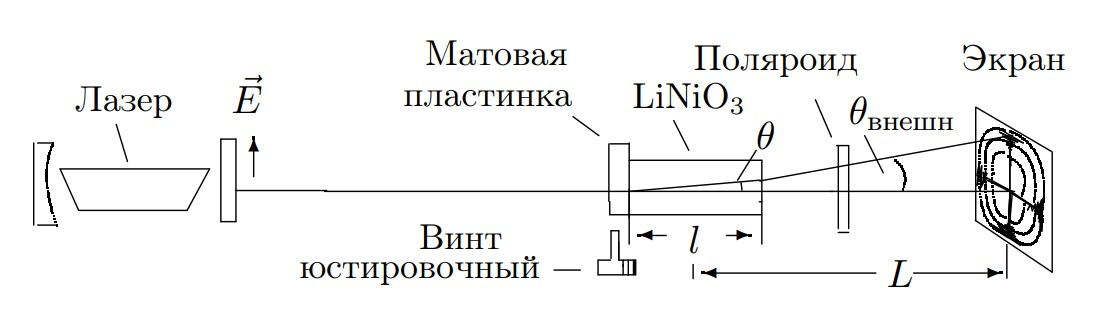
\includegraphics[scale=0.5]{1.jpg}
\caption{Оптическая часть экспериментальной установки}
\label{fig:image1}
\end{figure}

Если перед кристаллом, помещённым между поляроидами, расположить линзу или матовую пластинку, то на экране за поляроидом мы увидим тёмные концентрические окружности --- результат интерференции обыкновенной и необыкновенной волн.

При повороте выходного поляроида на $90^\circ$ картина меняется с позитива на негатив.

В случае, когда разрешённое направление анализатора перпендикулярно поляризации лазерного излучения, радиус тёмного кольца с номером $m$ равен

\[
r_m^2 =
\dfrac{\lambda}{l}
\dfrac{(n_o L)^2}{n_o - n_e}
m .
\]

\begin{figure}[h]
\centering
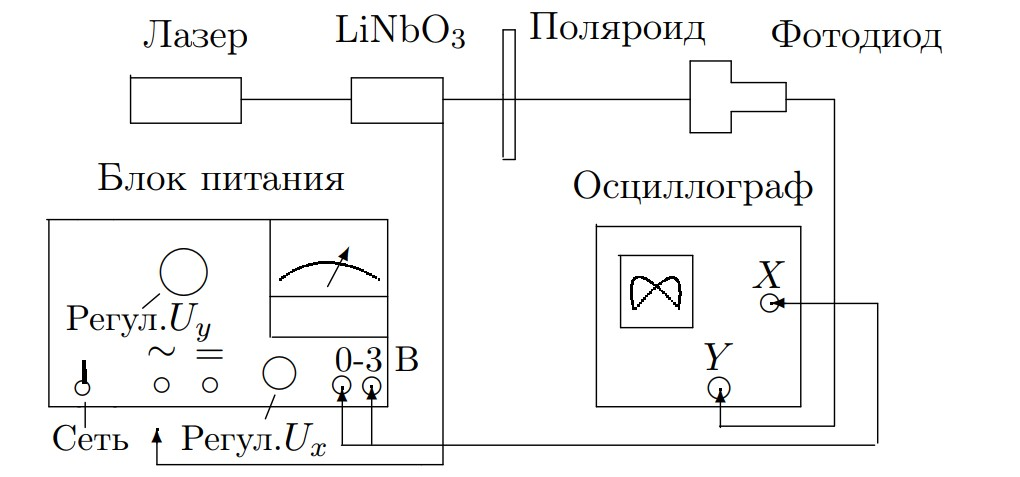
\includegraphics[scale=0.5]{2.jpg}
\caption{Экспериментальная установка}
\label{fig:image2}
\end{figure}

где $L$ --- расстояние от центра кристалла до экрана, $l$ --- длина кристалла.

Теперь поместим кристалл в постоянное электрическое поле $E_{\text{эл}}$, направленное вдоль оси $X$, перпендикулярной $Z$.

В плоскости $(X,Y)$ возникают два главных направления под углами $45^\circ$ к $X$ и $Y$ с показателями преломления $n_o-\Delta n$ и $n_o+\Delta n$.

\[
\Delta n = A E_{\text{эл}}
\]

Для поляризованного вертикально света и анализатора, пропускающего горизонтальную поляризацию:

\[
I_{\text{вых}} =
I_0
\sin^2
\left(
\dfrac{\pi}{2}
\dfrac{U}{U_{\lambda/2}}
\right)
\]

где

\[
U_{\lambda/2} =
\frac{\lambda}{4A}\frac{d}{l}
\]

--- \textit{полуволновое напряжение}.

\section{Ход работы}

\subsection{Интерференционная картина}
При прохождении лазерного луча через матовую платинку, кристалл и поляроид интерференционная картинка будет выглядить следующим образом: 

\begin{figure}[H]
\centering

\begin{minipage}{0.45\textwidth}
    \centering
    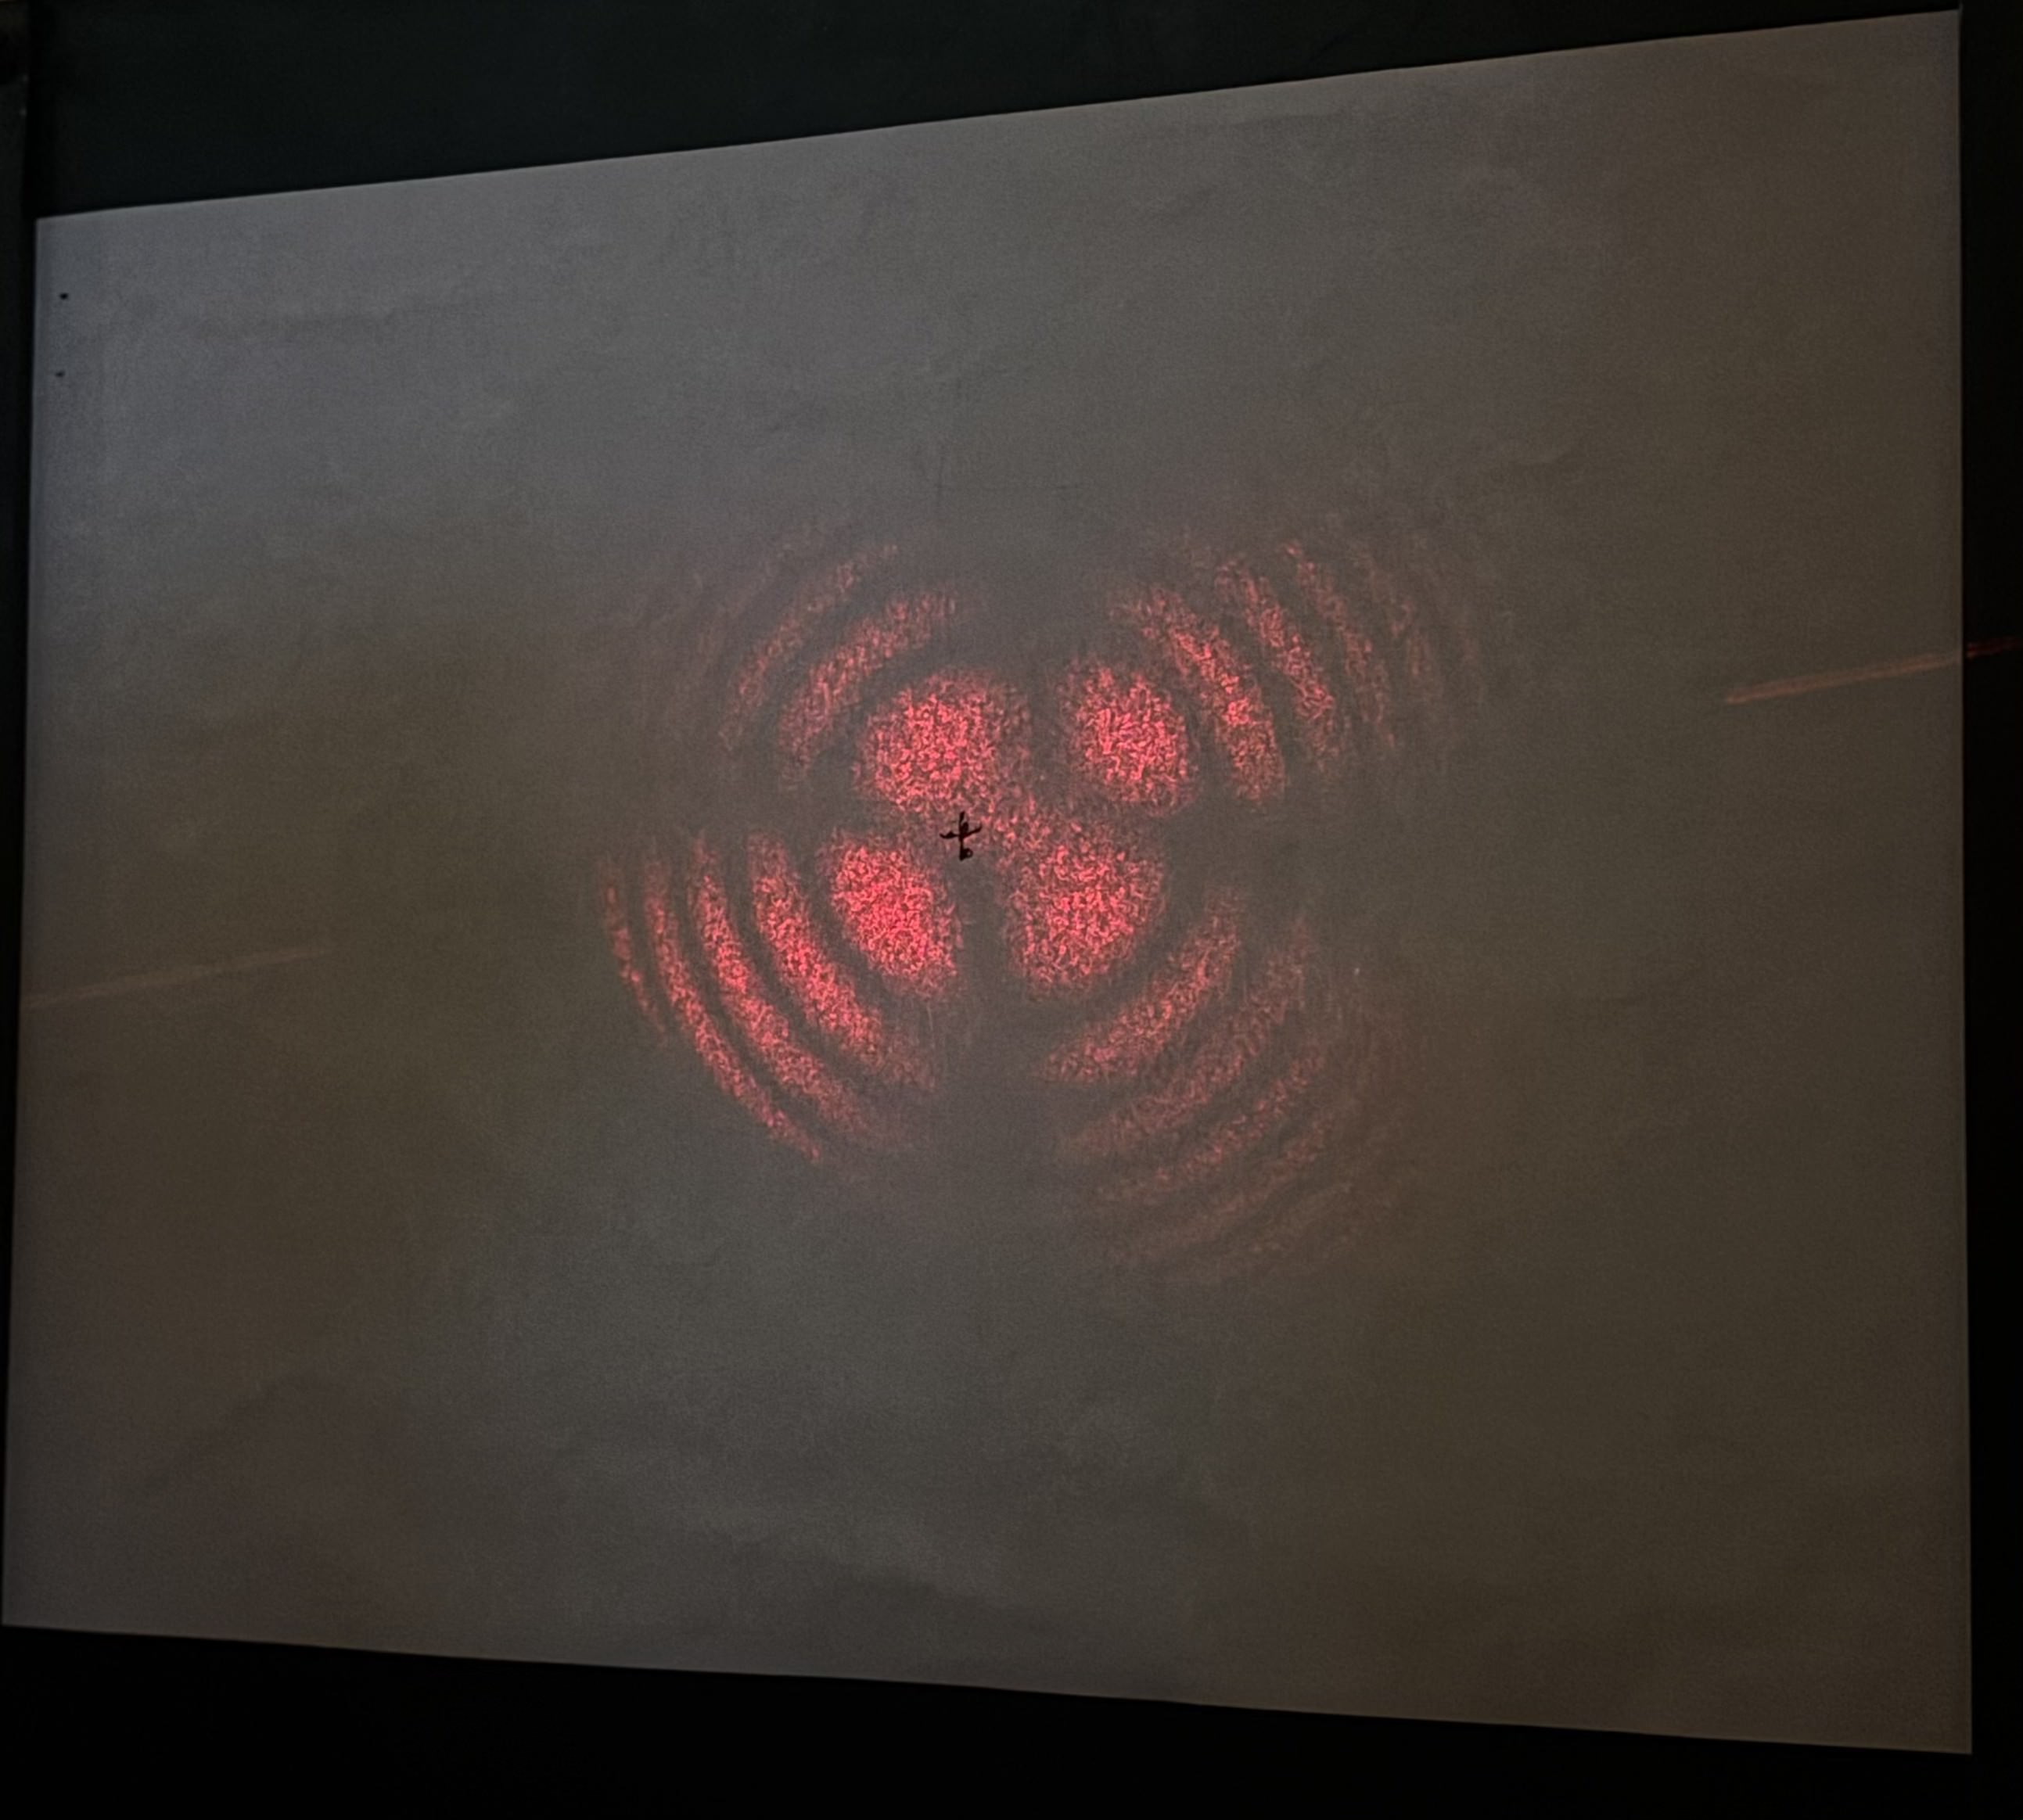
\includegraphics[width=\linewidth]{IMG_2639.jpg}
    \caption{Мальтийский крест}
\end{minipage}
\hfill
\begin{minipage}{0.45\textwidth}
    \centering
    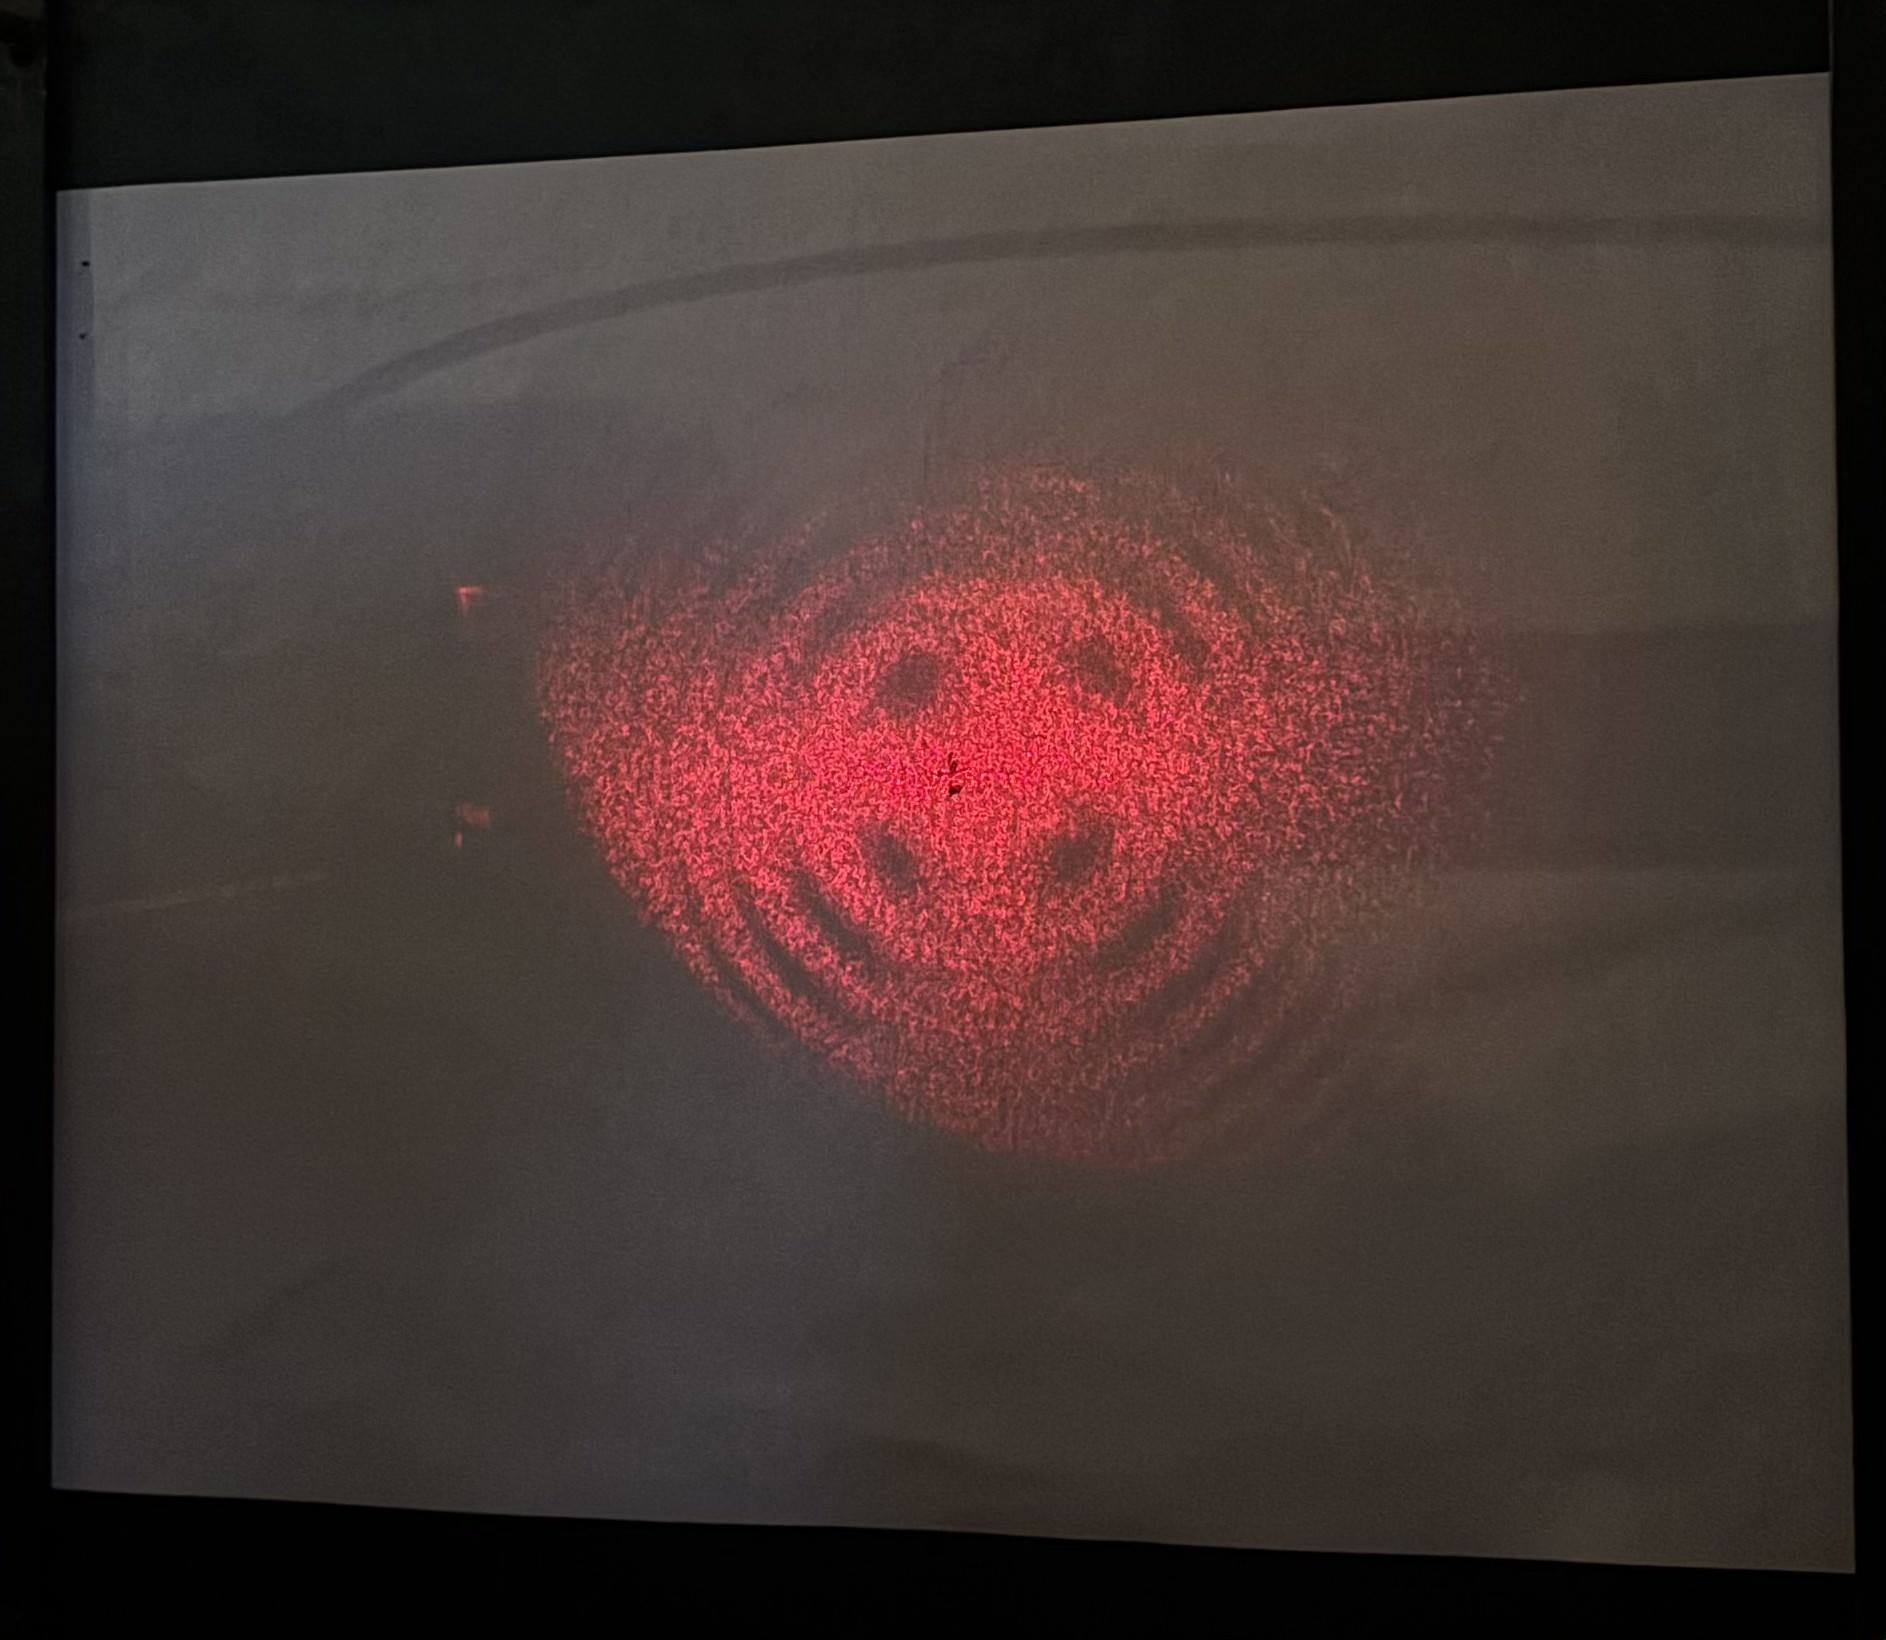
\includegraphics[width=\linewidth]{IMG_2640.jpg}
\end{minipage}

\end{figure}



Расстояние от середины кристалла до экрана

\[
L = 75 \pm 0.5 \text{ см}, \qquad
\lambda = 0.63 \text{ мкм}.
\]

Результаты измерений приведены в таблице:

\begin{center}
\begin{tabular}{|c|c|}
\hline
{$r^2$, см$^2$} & {$m$} \\
\hline
2.80 & 1 \\
4.00 & 2 \\
4.90 & 3 \\
5.60 & 4 \\
6.30 & 5 \\
6.90 & 6 \\
7.40 & 7 \\
8.00 & 8 \\
8.40 & 9 \\
\hline
\end{tabular}
\end{center}

По данным из таблицы 1 был построен график зависимости квадратов радиусов тёмных колец от номеров тёмных колец.

\begin{figure}[H]
    \centering
    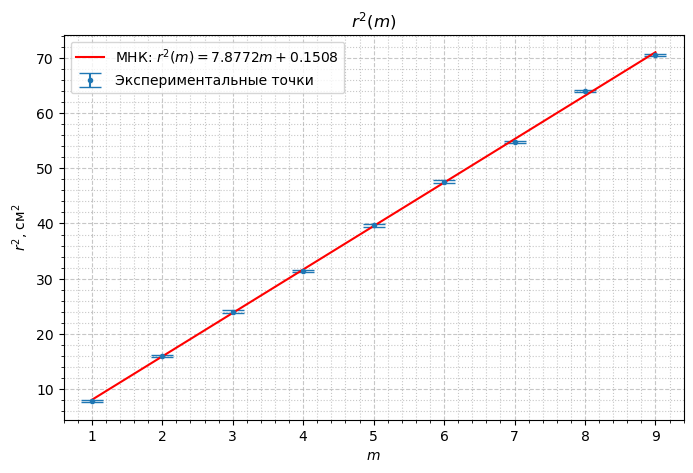
\includegraphics[width=0.65\linewidth]{r^2.png}
    \caption{Радиусы тёмных колец}
    \label{fig:placeholder}
\end{figure}

Полученное значение углового коэффициента $k = 7,9 \pm 0,2 \text{ см}^2$. Из формулы 2 получаем $$n_{o}-n_{e} = \dfrac{\lambda}{l} \dfrac{(n_oL)^2}{k} = 0,096 \pm 0,004$$. Это соотносится с табличным значением 0,09 в пределах погрешности.



\subsection{Определение полуволнового напряжения}
Если определять полуволновое напряжение по яркости пятна (яркость максимальна при $U = U_{\lambda/2}$ и минимальна при $U = U_{\lambda}$, то можно примерно установить значения этих напряжений. Проще всего увидеть наименее яркую точку, поэтому сначала определим полноволновое напряжение - его значение около 900 В ($\pm 30 $В). Можно заметить, что при значении напряжения в районе 450 В яркость точки сильно выше, чем при других значениях напряжений от 450 до 900 В. Значит, мы действительно измеряли полноволновое и полуволновое напряжение. При подаче 1350 В ($U = U_{3\lambda /2}$ можно заметить, как точка снова стала наименее яркой.\\
Проверим также, что при выставлении напряжения $U_{\lambda/4}$ получается круговая поляризация (интенсивность не меняется при вращении анализатора).\\
Если же определять полуволновое напряжение пр фигурам Лиссажу, полученным на осциллографе при помощи фотодиода, то получим следующие результаты:

\begin{figure}[H]
    \centering
    \begin{minipage}{0.33\linewidth}
        \centering
        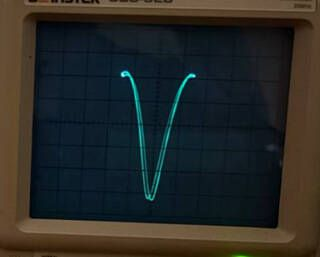
\includegraphics[width=\linewidth]{lis_half_2.jpg}
  
        \label{fig:image1}
    \end{minipage}
    \hfill
    \begin{minipage}{0.305\linewidth}
        \centering
        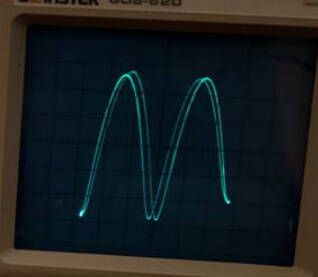
\includegraphics[width=\linewidth]{lis_full_2.jpg}

        \label{fig:image2}
    \end{minipage}
    \hfill
    \begin{minipage}{0.315\linewidth}
        \centering
        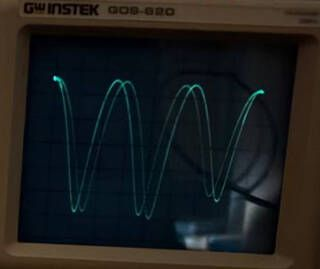
\includegraphics[width=\linewidth]{lis_1.5_2.jpg}
        \caption{Фигуры Лиссажу для полу-, полно- и четвертьволнового напряжения}
        \label{fig:image3}
    \end{minipage}
\end{figure}
$U_{\lambda/2} = 450 \pm15$B, $U_{\lambda} = 900 \pm 15$B, $U_{3\lambda/2} = 1350 \pm 15$B. В данном случае погрешность меньше, чем в предыдущем ($\pm 1$цена деления вместо $\pm 2$), так как возможно объективно определить, какое значение является искомым напряжением, с помощью формы фигуры Лиссажу на экране осциллографа.


Результаты измерений по ркости точки и при помощи фотодиода с осциллографом сходятся в пределах погрешности.

\section{Вывод}

В работе с помощью интерференционной картины было определено двулучепреломление ниобата лития.

Также был исследован эффект Поккельса и двумя способами определено полуволновое напряжение.

Полученные значения согласуются в пределах погрешности.

\section*{Выводы}

В ходе данной лабораторной работы было проведено исследование электрооптического эффекта Поккельса в кристалле ниобата лития ($\text{LiNbO}_3$).

\begin{itemize}
    \item В первой части работы получена и проанализирована интерференционная картина («Мальтийский крест»), возникающая при прохождении света через кристалл, помещенный между поляризатором и анализатором. На основе измерений радиусов тёмных интерференционных колец ($r_m$) построена зависимость $r^2(m)$.
    
    \item Используя угловой коэффициент полученной линейной зависимости ($k = 7,9 \pm 0,2 \text{ см}^2$), рассчитана величина двулучепреломления кристалла:
    \[
    n_o - n_e = \dfrac{\lambda}{l} \dfrac{(n_o L)^2}{k} = 0,096 \pm 0,004.
    \]
    Это значение хорошо согласуется с табличными данными ($\approx 0.09$), что подтверждает корректность проведенных наблюдений и расчетов.
    
    \item Во второй части работы определено полуволновое напряжение для используемого кристалла. Измерения проводились двумя способами: визуально по изменению яркости пятна и инструментально с помощью фотодиода и осциллографа (по фигурам Лиссажу).
    
    \item Полученные значения составили $U_{\lambda/2} = 450 \pm 15$ В,  $U_{\lambda} = 900 \pm 15$B, $U_{3\lambda/2} = 1350 \pm 15$B. Инструментальный метод, основанный на регистрации формы сигнала с фотодиода, позволил получить меньшую погрешность по сравнению с визуальной оценкой. Результаты, полученные обоими методами, совпадают в пределах погрешности.
    
    \item Также экспериментально подтверждено, что при напряжении $U_{\lambda/4}$ поляризация света становится круговой - при повороте анализатора (поляроида) яркость пятна не изменяется.
\end{itemize}

\end{document}